\documentclass[11pt, oneside]{article}   	% use "amsart" instead of "article" for AMSLaTeX format
\usepackage{geometry}                		% See geometry.pdf to learn the layout options. There are lots.
\geometry{letterpaper}                   		% ... or a4paper or a5paper or ... 
%\geometry{landscape}                		% Activate for rotated page geometry
%\usepackage[parfill]{parskip}    		% Activate to begin paragraphs with an empty line rather than an indent
\usepackage{graphicx}				% Use pdf, png, jpg, or eps§ with pdflatex; use eps in DVI mode
								% TeX will automatically convert eps --> pdf in pdflatex		
\usepackage{amssymb}
\usepackage[cache=false]{minted}
%SetFonts

%SetFonts


\title{Brief Article}
\author{The Author}
%\date{}							% Activate to display a given date or no date

\begin{document}
\begin{flushright}
Donovan Guelde\\
CSCI 5352\\
PS 6\\
\end{flushright}
1. a.\\
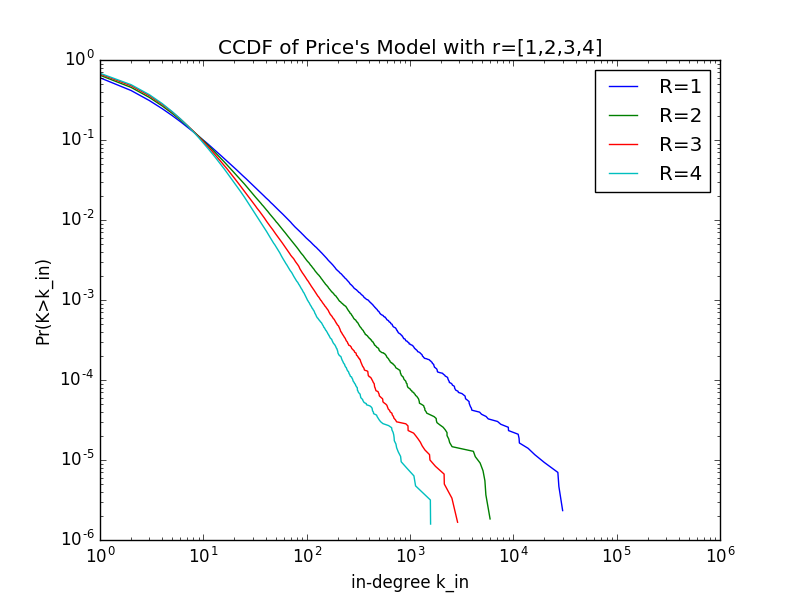
\includegraphics[scale=0.7]{1a_plot.png}\\\\
 \indent At low k\_in values less than 10, distributions of Price's model with varying R values are very similar.  In this area of the distribution, in-degree is primarily driven by random attachment.  At in-degree greater than 10, the R value becomes more important in determining in-degree, which can be seen in the separate distributions.  As R increases, the affect of preferential attachment decreases, causing a narrower distribution in in-degree.  After the 'shoulder' driven by random attachment, lower R values cause a more gradual drop-off in in-degree, reflecting a wider distribution.  Without preferential attachment, degree distribution would be much narrower, with a steeper drop-off in the CCDF plot (as seen in question 1.e.)\\
 \indent The opposite effect can be seen, to a small degree, for Pr(K$>$k\_in) where k\_in is less than 10.  At lower R values, the fraction of nodes with degree greater than 1 to 10 is higher than larger R values.  This is caused by the larger effect of random attachment.  Nodes that are added to the network towards the end of the growth period have an increased chance of being linked to by even later additions, as opposed to the preferential attachment model, which would give these 'late-comer' nodes a small chance of having an increased in-degree.  This explains the small but consistent trend at in-degree =0.  As the R value decreases, the fraction of nodes with in-degree = 0 also decreases.\\\\\\
 1.b.  Results were obtained using the simulation designed for 1.a. above, with c=12, R=5, and n=$10^6$.
 (i)  Averaging over 100 iterations, the average in-degree of the first 10\% (100,000) of papers published was determined to be 81.34.  The range of in-degree for the first 10\% of papers was quite large, with the largest average in-degree of 38,083.27, and the smallest in-degree of  17.11.\\
 (ii).  Average in-degree for the last 10\% of nodes added to the network was 0.187.  The largest average in-degree was 0.63, with many nodes having in-degree of zero.\\
 \indent To examine the first-mover advantage, we can examine the results for the first 10\% of papers more carefully.  The highest average in-degree is over 38,000, but moving down the sorted list of average in-degree just 13 places gives an average in-degree of 20,080.  By position 587, average in-degree is less than 1000.  The first-mover advantage definitely exists, and is limited to the small fraction of nodes added at the beginning of graph construction.  A similar examination of results for the last 10\% of papers published reveals a very small range, as previously mentioned.  A paper published in the last 90th percentile has very little advantage over even the very last paper published.\\\\\\
 1.c.  Average in-degree for the first 10\% of papers published in the "arXiv citation networks (1993-2003)" was determined to be 23.62, while the average in-degree for the last 10\% of papers published was 14.36.  These results do not agree with results from 1.b.  While there are more papers with relatively high in-degree in the first 10\% (over 100, for example), there are also many papers with low (less than 10) in-degree.  The extreme first-mover advantage seen in 1.b. is not present in this real network.  Results for the last 10\% of papers published also disagree with 1.b.  There are very few papers with 0 in-degree in the last 10\% of this network, in contrast to the many found in the simulation conducted in 1.b.\\
 \indent A possible explanation for absence of the extreme first-mover advantage seen in 1.b. could be that authors were not forced to rely solely on information and ideas presented in the early papers.  For example, the 10th paper published could be drawing on outside sources and independently formulating conclusions from the authors of the earlier papers.  In a new field, particularly, this may be common.  Many authors, while working in the same new field, draw from various sources.  This would reduce the first-mover advantage as other authors continue to publish.  Subsequent authors can also choose among the previously-published papers of highest quality.  This would give a small range of papers a high in-degree,  rather than just a few early-movers.\\\\\\
 1.d.  Ways that the preferential attachment mechanism is unrealistic are the extreme advantage given to first-movers, the extreme penalty given to late-comers, and the disregard for quality of work in a given paper, regardless of time published.  To analyze the first weakness of the preferential attachment model, the extreme first-mover advantage, we can perform analysis similar to 1.c. above.  A preferential attachment simulation shows a very strong first-mover advantage, while analysis of a real network does not bear this out.  There is definitely higher in-degree in earlier-published papers in the real network, but nowhere near as large as that predicted by simulation.  The extreme penalty for late-comers can be examined in a similar manner.  Simulations predict average in-degree of late-comers to be much less than 1, while real network examination in 1.c. does not agree.  To determine if quality of work, regardless of paper publishing date, one could look for outliers in both large and small expected in-degree.  The existence of a paper published in the very early stages of network growth, but with very low in-degree, could be an indicator of poor methodology or experiment design, among other things.  Similarly, a paper with very high in-degree among the last papers published could be an indicator of a breakthrough, interesting conclusions, etc. that allows the paper to gather many more citations than the preferential model would predict.\\\\\\
 1.e.  Removing the preferential attachment mechanism from our simulation used for 1.a. above acts to drastically reduce the distribution of node in-degree.  As seen in 1.a, the distribution of in-degrees narrows as R increases.  When preferential attachment is removed completely, we see the same 'shoulder' present in Price's model, but after that, the fraction of nodes with larger in-degree drops off very quickly to zero.  This plot completely lacks the power-log curve shown by Price's model.  The fraction of nodes with in-degree zero is smaller, since even the very last papers published have a higher chance of being cited without the preferential attachment mechanism.\\
 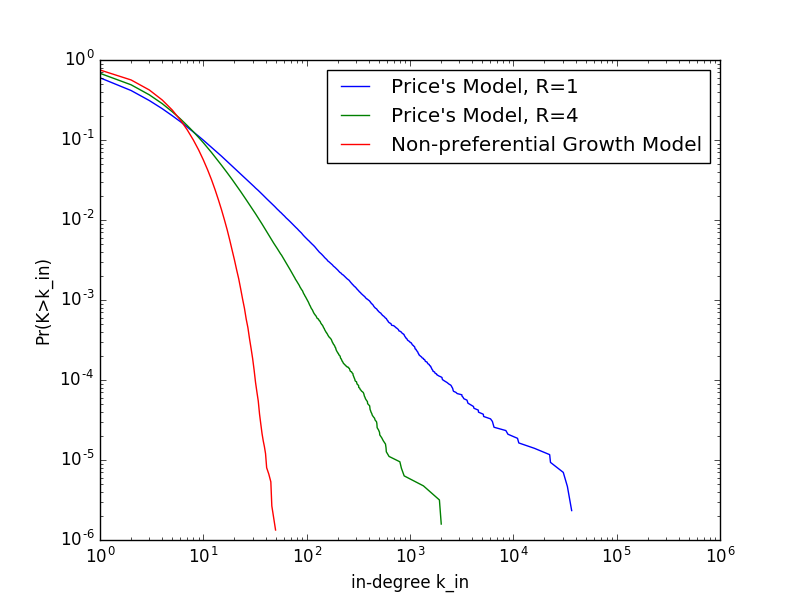
\includegraphics[scale=0.5]{1e}
 \\\\\\
 \begin{center}
 Code for 1.a.\\
\end{center}
\inputminted[linenos,fontsize=\scriptsize]{python}{q1a.py}
\begin{center}
 Code for 1.b.\\
\end{center}
\inputminted[linenos,fontsize=\scriptsize]{python}{q1b.py}
\begin{center}
 Code for 1.c.\\
\end{center}
\inputminted[linenos,fontsize=\scriptsize]{python}{q1c.py}
\begin{center}
 Code for 1.e.\\
\end{center}
\inputminted[linenos,fontsize=\scriptsize]{python}{q1e.py}



\end{document}  